\begin{frame}{Pictionary}
  \gloss{In groups of 4, take turns drawing pictures representing vocabulary items.
  Whoever is not drawing in the group should try to guess what it is.
  Whoever guesses first gets a point.
  Try to get the most points.
  \alert{The \lexi{dessinateur/dessinatrice} \gloss{drawer} can and should respond with \lexi{oui} or \lexi{non} followed by a complete sentence.}
  For example:}
  \begin{columns}
    \column{0.6\textwidth}
      \begin{description}
        \item[] (A picture of a marker is drawn by E1.)
        \item[E2:] Est-ce que c'est un stylo?
        \item[E1:] Non, ce n'est pas un stylo.
        \item[E3:] Est-ce que c'est un feutre?
        \item[E1:] Oui, c'est un feutre!
      \end{description}
    \column{0.4\textwidth}
      \begin{center}
        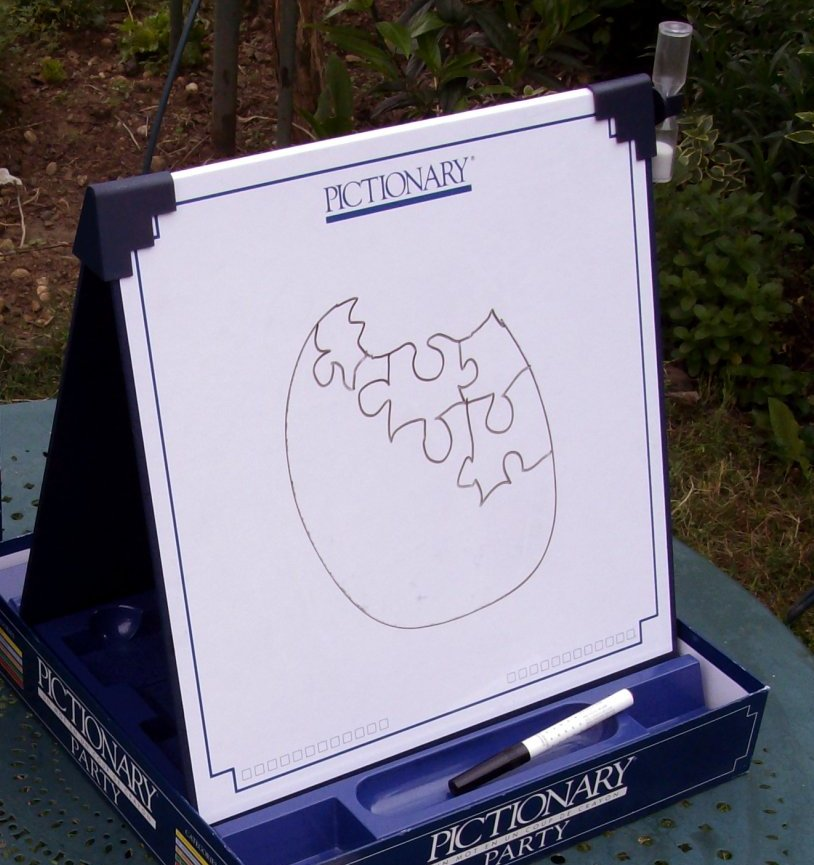
\includegraphics[scale=0.4]{pictionary.jpg}
      \end{center}
  \end{columns}
\end{frame}